% http://fachschaft.physik.uni-dortmund.de/images/GlobaltutAP/protokoll.txt
% ========================================
%	Header einbinden
% ========================================

% http://fachschaft.physik.uni-dortmund.de/images/GlobaltutAP/apheader.txt
% ==================================================
%	Festlegung der Dokumentenklasse
% ==================================================


\documentclass[paper=a4, 		% Layout für DinA4
	ngerman				% Deutsche Spracheinstellungen
	]
	{scrartcl} 			% Dokumentklasse für Aufsätze oder z.B. Praktikumsprotokolle

\usepackage{fixltx2e}			% Behebt ein paar Fehler in Latex

% ==================================================
%	Einstellen des Encodings
% ==================================================

\usepackage{ifxetex}
\usepackage{ifluatex} 

\ifxetex
	\usepackage{fontspec}
  	\usepackage{xunicode}
	\usepackage{xltxtra}
    \defaultfontfeatures{Mapping=tex-text} 	% To support LaTeX quoting style
	\setmainfont{Linux Libertine}
=======
    \defaultfontfeatures{Mapping=tex-text} % To support LaTeX quoting style
	\setmainfont{Linux Libertine} % Hier gewünschte Schriftart einfügen
\else
	\ifluatex
		\usepackage{fontspec}		% Falls das nicht funktioniert: \usepackage{luainputenc}
  		\usepackage{xunicode}
  		\defaultfontfeatures{Mapping=tex-text} % To support LaTeX quoting style
		\setmainfont{Linux Libertine} % Hier gewünschte Schriftart einfügen
	\else %pdfTeX
	  \usepackage[utf8]{inputenc}
	  \usepackage[T1]{fontenc}
	 \fi
\fi


% ==================================================
%	Spracheinstellungen
% ==================================================

\usepackage[ngerman]{babel,		% neue deutsche Rechtschreibung
	varioref}			% Bei Referenzen wird der Name des Objektes vor die Refernznummer geschrieben: z.B. \ref{bsp} liefert Seite 1

% ==================================================
%	Referenzen und Links
% ==================================================

\usepackage{hyperref}			% Verlinkungen innerhalb und außerhalb des PDF-Dokuments
\usepackage{url}			% Formattiert URLs, so dass sie sich z.B. besser vom Text abheben
\urlstyle{tt}				% TrueType-Schrift für URLs		



% ==================================================
%	Bibliograhphie
% ==================================================
%Zwei verschiedene Möglichkeiten Bibliographien einzubinden:

%	Möglichkeit 1:
% ========================
	\usepackage[numbers]{natbib}	%Paket für Bibliograhien

	%Bibtex: Nachnamen in Kapitälchen
	%\renewcommand*{\mkbibnamelast}[1]{\textsc{#1}}
	\newcommand*{\mkbibnamelast}[1]{\textsc{#1}}

	% Makros für Anhang + Referenzen
	\newcommand{\anhang}{
		\clearpage		% Anhang auf eine extra Seite packen
		\setcounter{page}{0}	
		\pagenumbering{Roman}	% Anhang wird in römischen Seitenzahlen numeriert
		\appendix		% Kapitelnummerierung in Großbuchstaben statt Zahlen.
	}

	\newcommand{\referenzen}{
		\bibliographystyle{alphadin} 			% Alphabetisch sortiert im DIN-Format
		\addcontentsline{toc}{section}{Referenzen}
		\phantomsection					% Referenzen ins Inhaltsverzeichnis
		\renewcommand{\refname}{\section*{Referenzen}\vspace*{-1em}} % Benennt das Kapitel um
		\bibliography{../include/Bibliographie.bib} 	% Die BibTeX-Datei einbinden
	}
%Zu Verwenden mit \bibliography{BIBDATEI}
% ========================
%	Möglichkeit 2:
% ========================
	%\usepackage{csquotes}				%Wird für Biblatex benötigt
	%\usepackage[style=alphabetic]{biblatex}	%Paket für Bibliograhphien mit Biblatex
%Zu Verwenden mit \bibliography{BIBDATEI} und \printbibliography oder \printbibliography[heading=bibintoc] (falls ein Inhaltsverzeichns verwendet wird)
% ==================================================



% ==================================================
%	Grafiken, Abbildungen und Tabellen
% ==================================================

\usepackage{graphicx}                   % zum Einbinden von Grafiken
\usepackage{xcolor}			% Für die Verwendung von Farben
\usepackage[font=small,			% kleine Schrift für Bildunterschriften
	labelfont=bf			% Fettgedruckte Bildunterschriften
	]
	{caption}			% Für Bildunterschriften

\usepackage{subcaption}			% Für mehrere Objekte nebeneinander mit eigenen Bildunterschriften

\usepackage{tabularx}			% Erweiterte Befehle für Tabellen
\usepackage{booktabs}			% Für professionele Tabellen, siehe Manual
\usepackage{longtable}			% Für Tabellen, die nicht mehr auf eine Seite passen.

\usepackage{rotating}			% Zum Verdrehen von Objekten. Nur mäßig verwenden.

%\graphicspath{{figs/}{bilder/}}	% Bildverzeichnisse MUSS ÜBERPRÜFT WERDEN!!!

% ==================================================
%	Mathematikumgebungen und Einheiten
% ==================================================

\usepackage{amsmath}			% Paket für mathematische Umgebungen und Funktionen
\usepackage{amsfonts}			% Zusätzliche Mathematische Schriftarten
\usepackage{amssymb}			% Zusätzliche Mathematische Symbole
%\usepackage{amscd}			% Zum Setzen Kommutativer Diagramme
\usepackage{amstext}			% Textsatz in der Matheumgebung
\usepackage{upgreek}			% Aufrechte griechische Buchstaben


% Diagramme mit tikz und Gnuplot zeichnen
%	\usepackage{tikz}
%	\usepackage{tikz-qtree}
%	\usepackage{gnuplot-lua-tikz}

% ==================================================
% SIUnitX: Einheiten werden vollautomatisch gesetzt
% ==================================================
\usepackage[
    separate-uncertainty = true, 		% Stellt den Fehler separat dar: Siehe SIUnitX-Manual
    mode 			= text, 	% Stellt Einheiten (Kelvin etc.) Nichtkursiv dar
    quotient-mode	= 	fraction,	% Bruchstriche nutzen
    repeatunits           = false, 
    range-phrase          = {\,bis\,},  
]{siunitx}
\sisetup{
	per-mode = fraction, 			% Bruchstriche nutzen
	output-decimal-marker = {,}, 		% Setzt das Dezimaltrennzeichen als Komma
	multi-part-units = brackets,
	exponent-product = \cdot,
}

\addto\extrasgerman{\sisetup{locale = DE}}	% "Deutsche" Einheiten
\usepackage{cancel}				% Kürzen von Einheiten in SIUnitX ermöglichen


% ==================================================
%	Sonstiges
% ==================================================

%\usepackage[official]{eurosym}			% offizielles Eurosymbol

% ==================================================
%	Seitenlayout
% ==================================================

% Kein Einrücken der Absätze (Einrücken = Null)
	\setlength{\parindent}{0pt}             % kein Einrücken der ersten Zeile in einem neuen Absatz

% Vermeidung von "Schusterjungen"
	\clubpenalty = 3000			% Höchstwert 10000, dann dürfen theoretisch keine Schusterjungen mehr auftreten.
% Vermeidkung von "Hurenkindern"
	\widowpenalty = 3000			% Höchstwert 10000, dann dürfen theoretisch keine Hurenkinder mehr auftreten.
	\displaywidowpenalty = 3000		% Es werden beide Einstellungen benötigt.

% Seitenlayout ändern mit Fancy
	\usepackage{fancyhdr}			% Paket zum bequemeren Verändern des Seitenlayouts

	% Tabellen ändern:
		\renewcommand{\thetable}{\arabic{section}.\arabic{table}} % figures bekommen die richtige Nummerierung: x.y
		\makeatletter \@addtoreset{table}{section} \makeatother      % nach jeder section wird neu gezählt

	% Kapitelüberschriften in der Kopfzeile:
		\renewcommand*{\sectionmark}[1]{\markboth{}{\thesection\ #1}}
		%\renewcommand*{\subsectionmark}[1]{\markboth{}{\thesubsection\ #1}}
		\renewcommand*{\subsectionmark}[1]{\markboth{}{}} % keine Unterüberschriften in der Kopfzeile
		\renewcommand{\plainheadrulewidth}{0.4pt}
	
	% Seitennummern rechts in der Kopfzeile:
		\lhead[\fancyplain{\thepage}{\thepage}]{\fancyplain{}{\rightmark}}
		\rhead[\fancyplain{}{\leftmark}]{\fancyplain{\thepage}{\thepage}}
	
	%Fußzeilen bleiben leer
		\lfoot{}
		\cfoot{}
		\rfoot{}
		
%Eigenes
\usepackage[section]{placeins} %use \FloatBarrier to keep pictures or tables in front of barrier
\renewcommand*\rmdefault{iwona}\normalfont\upshape

% ========================================
%	Angaben für das Titelblatt
% ========================================

\title{Versuch 500 - Der Photoeffekt\\				% Titel des Versuchs 
\large TU Dortmund, Fakultät Physik\\ 
\normalsize Anfänger-Praktikum}

% \author{Marc Posorske\\			% Name Praktikumspartner A
% {\small \href{marc.posorske@tu-dortmund.de}{marc.posorske@tu-dortmund.de}}	% Erzeugt interaktiven einen Link
% \and						% um einen weiteren Author hinzuzfügen
% Fabian Lehmann\\					% Name Praktikumspartner B
% {\small \href{fabian.lehmann@tu-dortmund.de}{fabian.lehmann@tu-dortmund.de}}		% Erzeugt interaktiven einen Link
% }

% \author{Fabian Lehmann\\					% Name Praktikumspartner B
% {\small \href{fabian.lehmann@tu-dortmund.de}{fabian.lehmann@tu-dortmund.de}}		% Erzeugt interaktiven einen Link
% }

\author{Oliver Zietek\\			% Name Praktikumspartner A
{\small \href{oliver.zietek@tu-dortmund.de}{oliver.zietek@tu-dortmund.de}}	% Erzeugt interaktiven einen Link
\and						% um einen weiteren Author hinzuzfügen
Fabian Lehmann\\					% Name Praktikumspartner B
{\small \href{fabian.lehmann@tu-dortmund.de}{fabian.lehmann@tu-dortmund.de}}		% Erzeugt interaktiven einen Link
}

\date{10. Januar 2013}%21.Dezember 2012}				% Das Datum der Versuchsdurchführung

% ========================================
%	Das Dokument beginnt
% ========================================

\begin{document}

% ========================================
%	Titelblatt erzeugen
% ========================================

\maketitle					% Jetzt wird die Titelseite erzeugt
\thispagestyle{empty} 				% Weder Kopfzeile noch Fußzeile

% ========================================
%	Der Vorspann
% ========================================

%\newpage					% Wenn Verzeichnisse auf einer neuen Seite beginnen sollen
%\pagestyle{empty}				% Weder Kopf- noch Fußzeile für Verzeichnisse

\tableofcontents

%\newpage					% eine neue Seite
%\thispagestyle{empty}				% Weder Kopf- noch Fußzeile für Verzeichnisse
%\listoffigures					% Abbildungsverzeichnis

%\newpage					% eine neue Seite
%\thispagestyle{empty}				% Weder Kopf- noch Fußzeile für Verzeichnisse
%\listoftables					% Tabellenverzeichnis
\newpage					% eine neue Seite


% ========================================
%	Kapitel
% ========================================

%\section{Einleitung}				% Bei Bedarf
%	%
%
In diesem Versuch werden die mit dem lichtelektrischen Effekt zusammenh"angenden Erscheinungen
quantitativ untersucht werden. Eine dieser Erscheinungen ist die Abhängigkeit der
Elektonenenergie von der Wellenlänge des Lichts, welche in diesem Versuch bestätigt werden
soll.
\section{Theorie}
	%
%
\subsection{Die Natur des Lichts}
Es gibt zwei Vorstellungen zur Natur des Lichtes. Die eine ist die Wellentheorie, die andere
die korpuskulare Theorie. Diese Beiden scheinen auf den ersten Blick unvereinbar in der mathematischen
Beschreibung, welche einmal durch die Maxwellgleichungen (Wellentheorie) und ein anderes
mal durch die newtonsche Punktmechanik(korpuskulare Theorie) beschrieben werden. Es ist auch nur in der Quantenmechanik
möglich eine vollständig Beschreibung zu geben. Hier treten dann die beiden
Modelle als Grenzfälle auf.
Welches Modell nun zutrifft, hängt immer von dem Experiment ab.
So wird die Wellentheorie bei Beugung am Spalt oder Inteferenz benutzt und die Korpuskel beim lichtelektrichen
Effekt oder Comptoneffekt. Es l"asst sich also allgemein sagen, dass bei einer großen Anzahl an
Photonen, die man über die räumliche Ausbreitung mittelt, die Wellentheorie nimmt und
bei Wechselwirkungen mit Materie und Licht das Korpuskullmodell.

\subsection{Der Photoeffekt}
Es wird eine sich im Vakuum befindliche Festkörperoberfläche mit monochromatischem
Licht bestrahlt. Dieser Körper wird Photokathode genannt. Es wird der gegebenüber stehenden Elektrode
ein höheres Potential zugeteilt, damit die Elektronen von der Photokathode zu dieser gelenkt werden.
Es folgen die Ergebnisse:
 \begin{description}

\item[Die Zahl der pro Zeiteinheit ausgelösten Elektronen ist proportional zur Lichtintensität.]

\item[Eine Grenzfrequenz, unter welcher der Photoeffekt nicht mehr auftrit, existiert.]

\item[Die Energie der Photoelektronen (gemessen über ihre Geschwindigkeit) ist proportional zur Lichtfrequenz und unabhängig von der Lichtintensität.]

 \end{description}

Sämtliche Ergebnisse lassen sich nicht mit einem Wellenmodell erklären:
Wenn man beispielsweise annimmt, dass die Elektronen an der Oberfläche eines Metalles durch das elektrische Feld des einfallenden Lichtes zu erzwungenen Schwingungen angeregt werden, dann müssten die Elektronen die Metalloberfläche verlassen können, sobald ihre Schwingungsamplitude so groß geworden ist, dass sie die elektrostatischen, rück-treibenden Kräfte überwinden. Das heißt, dass auch bei langwelligem Licht mit ausreichend hoher Intensität der Photo-Effekt möglich sein müsste. Es müsste bei einer bestimmten Frequenz Resonanzphänomene zu beobachten sein, wo der Photo-Effekt bevorzugt auftritt. Weiterhin müsste die Energie der Photoelektronen mit der Lichtintensität anwachsen. All diese Forderungen stehen aber im Widerspruch zu den experimentellen Ergebnissen.

Mit dem korpuskel Modell kann man aber all diese Punkte erklären, denn ein Photon der Frequenz
$\nu$ hat eine Engergie von $h \nu$, wenn diese Energie gleich oder größer der Austrittsarbeit $A_k$ eines Elektron ist,
da das Photon diese übergibt, löst sich das Elektron aus dem Festkörper mit einer Geschwindigkeit, die aus $E_{kin}$ herrührt.
So kann man diese Gleichung aufstellen:
\begin{align}
h \nu = E_{kin} + A_k
\end{align}
Dies erklärt große Teile der Ergebnisse. Es ist nocht anzumerken, dass ein Photon nur ein Elektron lösen kann. Folglich sind die ausgelösten Elektronen proportional zur Lichtintensität.

\begin{figure}[h]
	\centering
		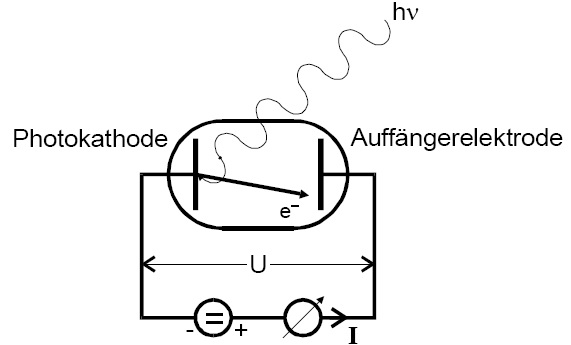
\includegraphics[width=1.00\textwidth]{PrinzipDesPhotoeffekts.jpg}
		\caption{Prinzip des Photoeffekts}
	\label{fig:PrinzipDesPhotoeffekts}
\end{figure}
	\FloatBarrier
\section{Durchführung}
	%
%picaufbau
\subsection{Versuchsaufbau}
	\begin{figure}[h]
		\begin{center}
		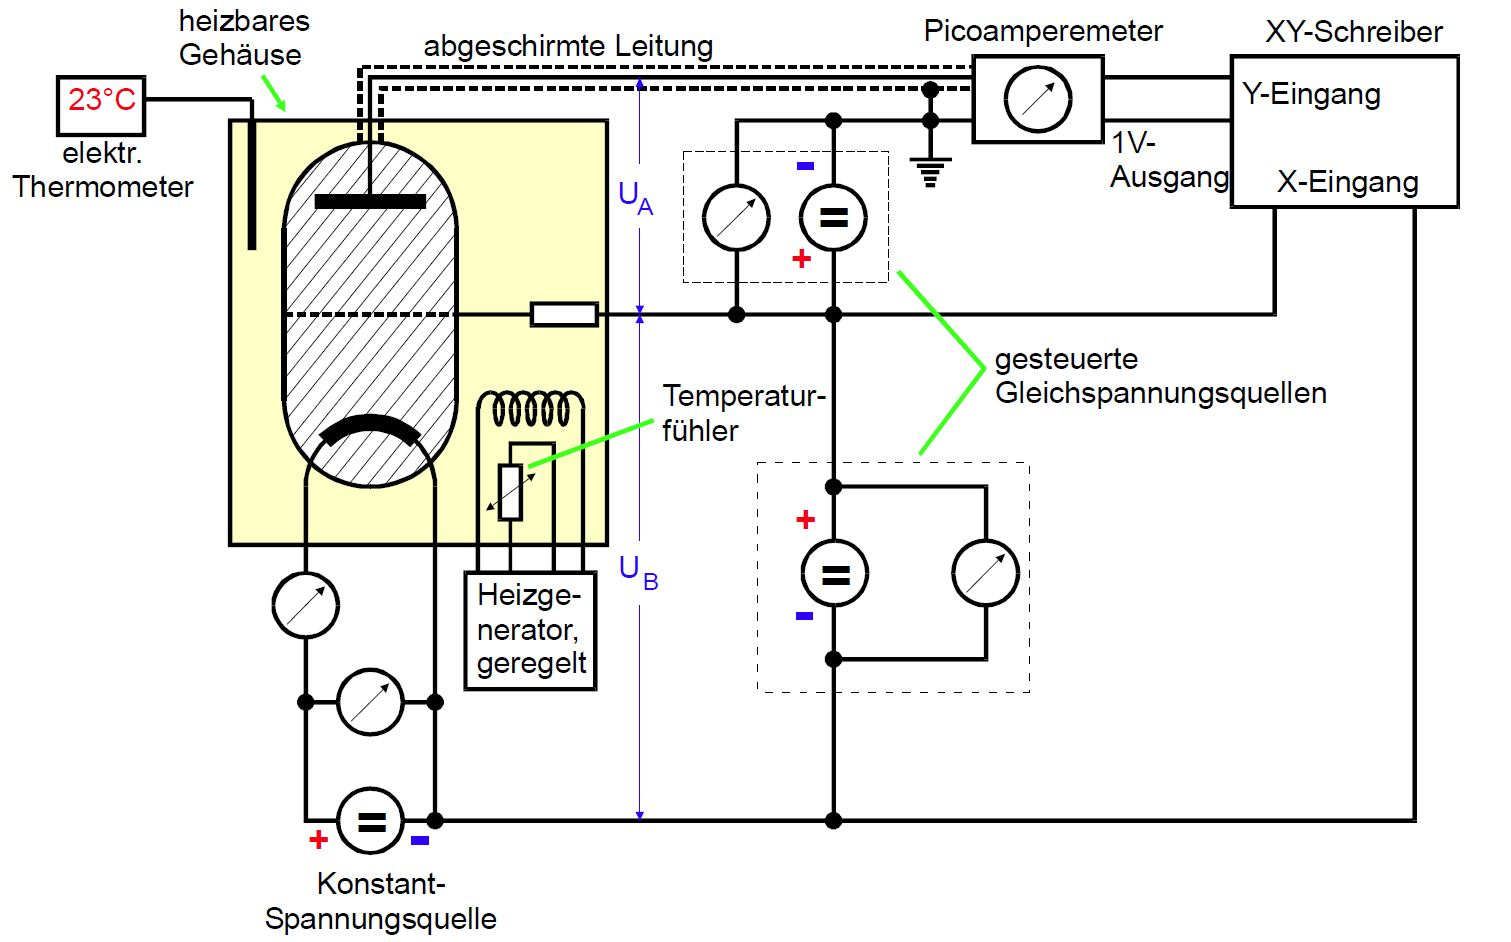
\includegraphics[scale=0.3]{picaufbau.jpg}
		\caption{Versuchsschaltung [1]}
		\label{picaufbau}
		\end{center}	
	\end{figure}
Der Versuch wird wie in Abbildung \ref{picaufbau} aufgebaut, sodass
die Aufnahmen für die folgenden Versuchsteile aufgezeichnet werden können.
\subsection{Betimmung der Energieverteilung der beschleunigten Elektronen}
Nachdem der X-Y-Schreiber auf das aufzuzeichnende Intervall kalibriert ist, wird
bei konstantem Beschleunigungsstrom und
bei Zimmertemperatur, beziehungsweise bei erhöhter Temperatur
jeweils der Auffängerstrom in Abhängigkeit der Abbremsspannung aufgezeichnet.
\subsection{Bestimmung der Franck-Hertz-Kurve}
Nachdem der X-Y-Schreiber auf das aufzuzeichnende Intervall kalibriert ist, wird
bei passender Temperatur und konstanter Abbremsspannung der Auffängerstrom in 
Abhängigkeit der Beschleunigungsspannung 
aufgezeichnet, sodass deutlich genug Maxima zu erkennen sind.
\subsection{Bestimmung der Ionisierungsspannung von Hg}
Nachdem der X-Y-Schreiber auf das aufzuzeichnende Intervall kalibriert ist, wird
bei hoher Abbremsspannung und erhöhter Temperatur der Auffängerstrom in Abhängigkeit 
der Beschleunigungsspannung aufgezeichnet.
	\FloatBarrier
\section{Auswertung}
	%NEEDSequg
%tabspektrum, tabaall, tabay, tabug, tabalinreg, picaALL, picavio2lin, picavio1lin, picagrunlin, picagelblin, picablaugrunlin, picblinreg1

\subsection{Bestimmung von $U_g$} %Abhängigkeit des Photostromes von Bremsspannung}
\begin{table}[h]
	\begin{center}
		\begin{tabular}{ccc}
			$\lambda$/nm&Farbe&$\nu \cdot 10^{(14)}$/$\frac{1}{\text{s}}$ \\ \hline
			405&Violett&7,40\\
			435&Violett&6,89\\
			492&Grün&6,09\\
			546&Blaugrün&5,49\\
			578&Gelb&5,19
		\end{tabular}
		\caption{Untersuchte Linien des Hg-Spektrums[1]}
		\label{tabspektrum}
	\end{center}
\end{table} \begin{table}[h]
	\begin{center}
		\begin{tabular}{c|cccc}
			$U$/V&405nm: I/nA&435nm: I/nA&492nm: I/nA&546nm: I/nA \\ \hline
			-1,0&	0,027& 0,000&0,000&-0,018\\
			-0,8&	0,097& 0,094&0,000&-0,016\\
			-0,6&	0,225& 0,280&0,003&-0,011\\
			-0,4&	0,400& 0,720&0,012& 0,011\\
			-0,2&	0,630& 1,100&0,030& 0,140\\
			 0,0&	0,840& 1,350&0,054& 0,460\\
			 0,2&	1,050& 2,050&0,080& 0,830\\
			 0,4&	1,350& 2,550&0,105& 1,200\\
			 0,6&	1,650& 3,100&0,135& 1,500\\
			 0,8&	1,900& 3,600&0,155& 1,800\\
			 1,0&	2,200& 4,000&0,175& 2,050\\
			 5,0&	7,200&12,500&0,530& 5,600\\
			 9,0&  10,000&17,500&0,720& 7,000\\
			13,0&  12,000&20,500&0,820& 7,800\\
			17,0&  13,500&22,500&0,870& 8,200\\
			19,0&  14,000&23,000&0,930& 8,700
		\end{tabular}
		\caption{Photostrom verschiedener Wellenlängen in Abhängigkeit der Spannung}
		\label{tabaall}
	\end{center}
\end{table} \begin{table}[h]
	\begin{center}
		\begin{tabular}{cc}
			$U_g$/V&I/nA \\ \hline
			-19,0&-0,010\\
			-17,0&-0,012\\
			-13,0&-0,011\\
			 -9,0&-0,009\\
			 -5,0&-0,009\\
			 -1,0&-0,008\\
			 -0,8&-0,006\\
			 -0,6&-0,004\\
			 -0,4&0,000\\
			 -0,2&0,018\\
			  0,0&0,120\\
			  0,2&0,290\\
			  0,4&0,460\\
			  0,6&0,610\\
			  0,8&0,720\\
			  1,0&0,880\\
			  5,0&1,800\\
			  9,0&2,200\\
			 13,0&2,350\\
			 17,0&3,800\\
			 19,0&4,000
		\end{tabular}
		\caption{Photostrom in Abhängigkeit der Spannung ($\lambda=578$ nm)}
		\label{tabay}
	\end{center}
\end{table} 	\begin{figure}[h]
		\begin{center}
		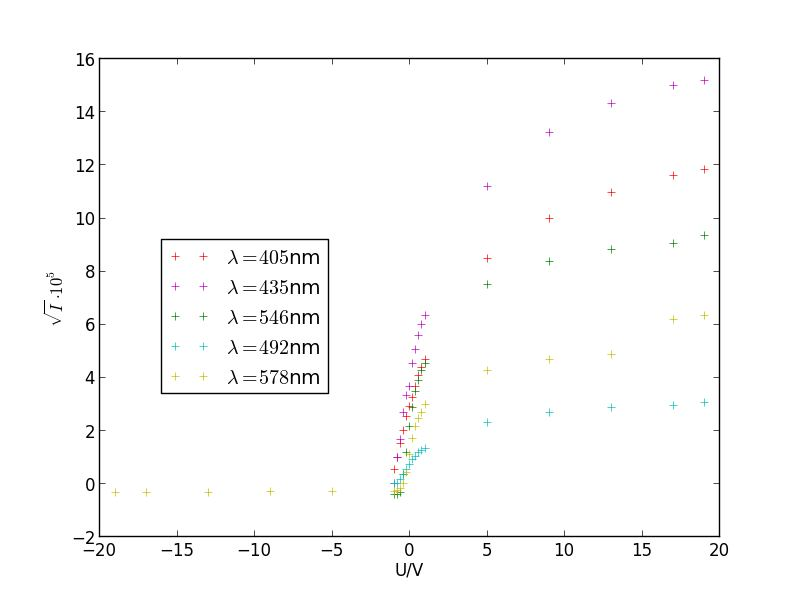
\includegraphics[scale=0.7]{picaALL.jpg}
		\caption{Photostrom in Abhängigkeit der angelegten Spannung}
		\label{picaALL}
		\end{center}	
	\end{figure}
	\begin{figure}[h]
		\begin{center}
		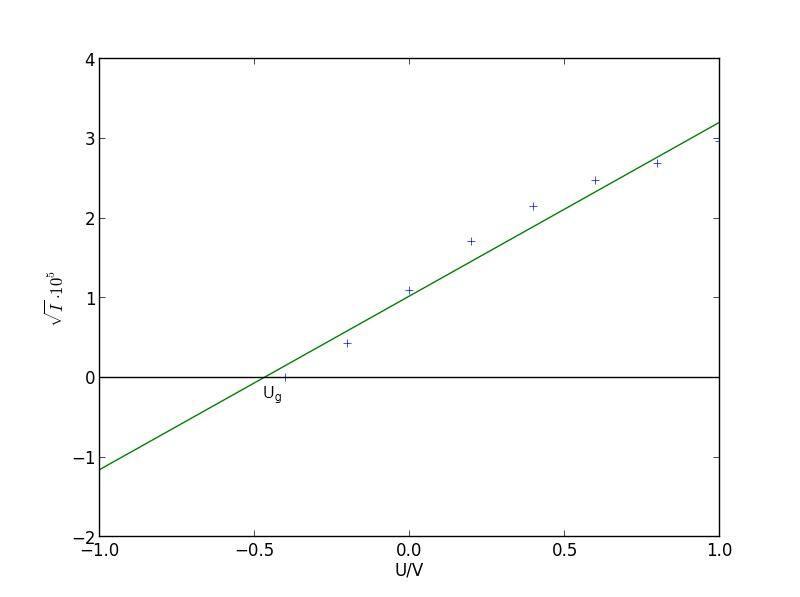
\includegraphics[scale=0.7]{picagelblin.jpg}
		\caption{Lineare Regression des Photostroms ($\lambda=578$ nm)}
		\label{picagelblin}
		\end{center}	
	\end{figure} 	\begin{figure}[h]
		\begin{center}
		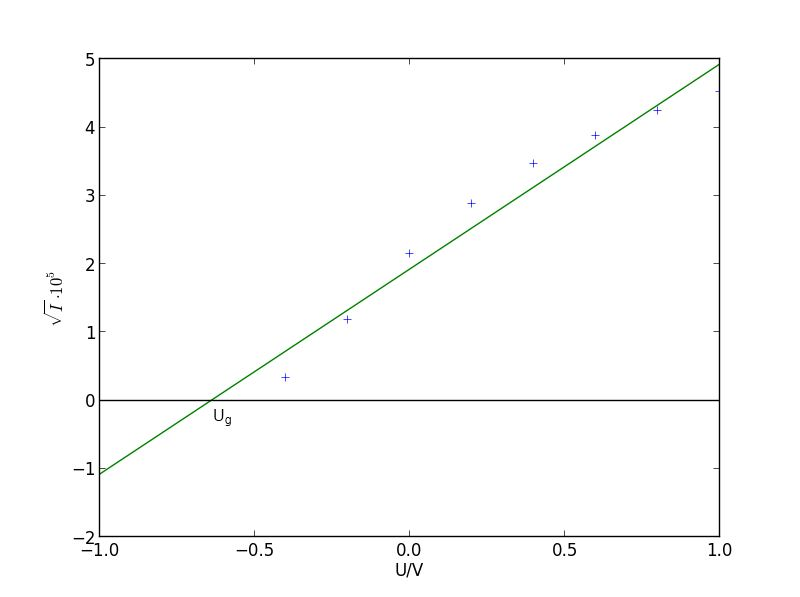
\includegraphics[scale=0.7]{picagrunlin.jpg}
		\caption{Lineare Regression des Photostroms ($\lambda=546$ nm)}
		\label{picagrunlin}
		\end{center}	
	\end{figure} 	\begin{figure}[h]
		\begin{center}
		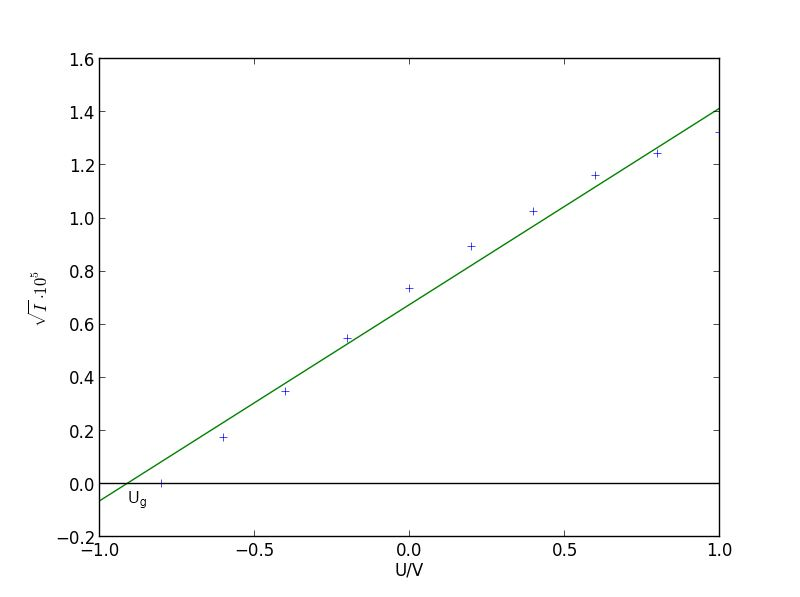
\includegraphics[scale=0.7]{picablaugrunlin.jpg}
		\caption{Lineare Regression des Photostroms ($\lambda=492$ nm)}
		\label{picablaugrunlin}
		\end{center}	
	\end{figure} 	\begin{figure}[h]
		\begin{center}
		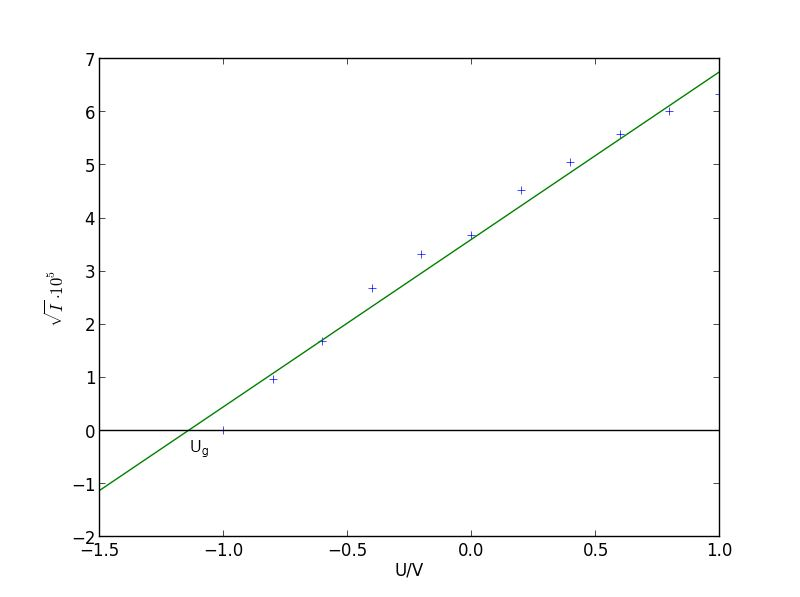
\includegraphics[scale=0.7]{picavio1lin.jpg}
		\caption{Lineare Regression des Photostroms ($\lambda=435$ nm)}
		\label{picavio1lin}
		\end{center}	
	\end{figure} 	\begin{figure}[h]
		\begin{center}
		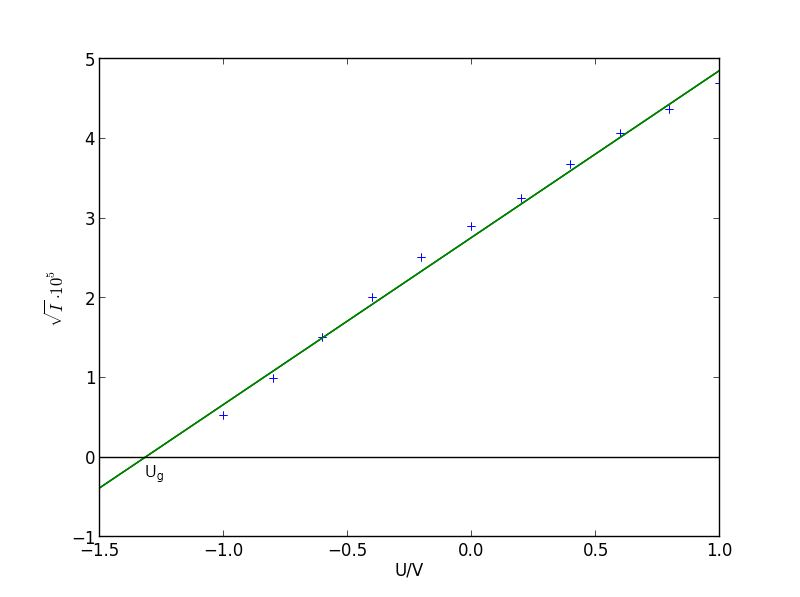
\includegraphics[scale=0.7]{picavio2lin.jpg}
		\caption{Lineare Regression des Photostroms ($\lambda=405$ nm)}
		\label{picavio2lin}
		\end{center}	
	\end{figure}
\begin{table}[h]
	\begin{center}
		\begin{tabular}{c|cc}
			$\lambda$/nm&a$\cdot 10^{-5}$&b$\cdot 10^{-5}$ \\ \hline
			405&2,10$\pm$0,06&2,77$\pm$0,04\\
			435&3,15$\pm$0,14&3,62$\pm$0,09\\
			492&0,74$\pm$0,03&0,68$\pm$0,02\\
			546&3,00$\pm$0,25&1,93$\pm$0,14\\
			578&2,18$\pm$0,16&1,03$\pm$0,09
		\end{tabular}
		\caption{Ergebnisse der linearen Regression}
		\label{tabalinreg}
	\end{center}
\end{table} \begin{table}[h]
	\begin{center}
		\begin{tabular}{cc}
			$U_g$/V&$\lambda$/nm \\ \hline
			-1,3202&405\\
			-1,1471&435\\
			-0,9163&492\\
			-0,6430&546\\
			-0,4733&578
		\end{tabular}
		\caption{$U_g$ in Abhängigkeit der Wellenlänge}
		\label{tabug}
	\end{center}
\end{table}
%\FloatBarrier
Wird die Wurzel aus dem Photostrom gegen die Bremsspannung aufgetragen, so lässt sich
für die verschiedenen Wellenlängen (vgl. Tab. \ref{tabspektrum}) aus den Tabellen \ref{tabaall} und \ref{tabay} Abbildung \ref{picaALL}
erstellen. Wird nun für die linearen Abschnitte aus Abbildung \ref{picaALL} jeweils eine lineare 
Regression \cite{linreg} durchgeführt (siehe Tab. \ref{tabalinreg}), 
\begin{align}
\sqrt{I}&=a\cdot U+b,
\end{align}
so lassen
sich aus dem Schnittpunkt der Ausgleichsgeraden mit der Spannungs-Achse (Abb. \ref{picagelblin} - 
\ref{picavio2lin}) die Gegenspannungen $U_g$ bestimmen.
\begin{align}
U_g&=\frac{-b}{a}
\end{align}

\subsection{Bestimmung der Austrittsarbeit und des Verhältnisses $\frac{h}{e_0}$}
	\begin{figure}[h]
		\begin{center}
		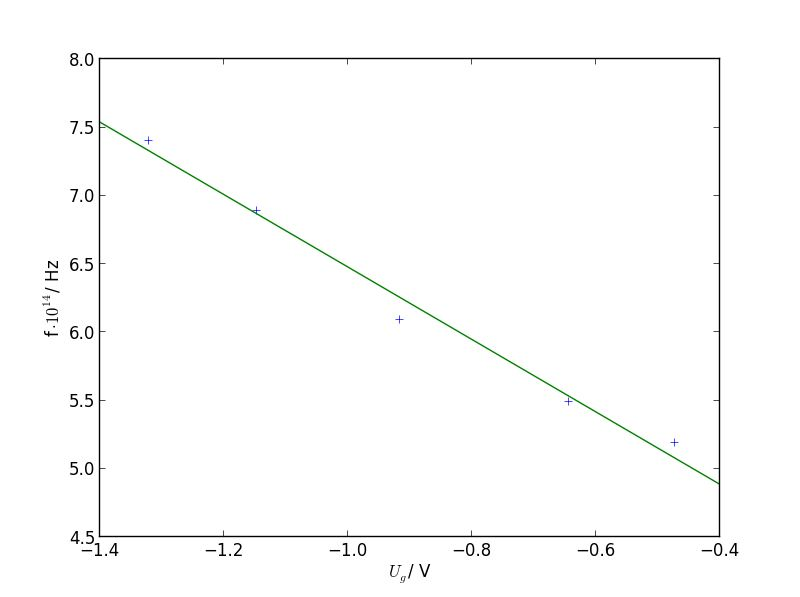
\includegraphics[scale=0.7]{picblinreg1.jpg}
		\caption{Lineare Regression von $U_g$ bezogen auf die Lichtfrequenz}
		\label{picblinreg1}
		\end{center}	
	\end{figure}
Wird $U_g$ (Tab. \ref{tabug}) gegen die Lichtfrequenz (Tab. \ref{tabspektrum}) aufgetragen 
(Abb. \ref{picblinreg1}) und dann ein lineare Regression \cite{linreg} durchgeführt, so 
lassen sich Austrittsarbeit $A_k$ und das Verhältnis $\frac{h}{e_0}$ mit Gleichung (\ref{equg}) 
bestimmen.
\begin{align}
\nu &= \frac{e_0}{h} |U_g| + \frac{A_k}{h}\\
\frac{A_k}{h}&=(3,8\pm0,2)\cdot10^{14}\text{ }\frac{1}{s}\\
\Rightarrow A_k&=(1,58\pm0,07)\text{ eV}\\
\frac{h}{e_0}&=((2,6 \pm 0,2)\cdot 10^{14} \text{ } \frac{\text{C}}{\text{J}\cdot \text{s}})^{-1}=(3,8\pm0,3)\cdot10^{-15}\text{ }\frac{\text{J$\cdot$s}}{\text{C}}
\end{align}


% \subsection{Deutung eines Kurvenverlaufs}
% 	\begin{figure}[h]
		\begin{center}
		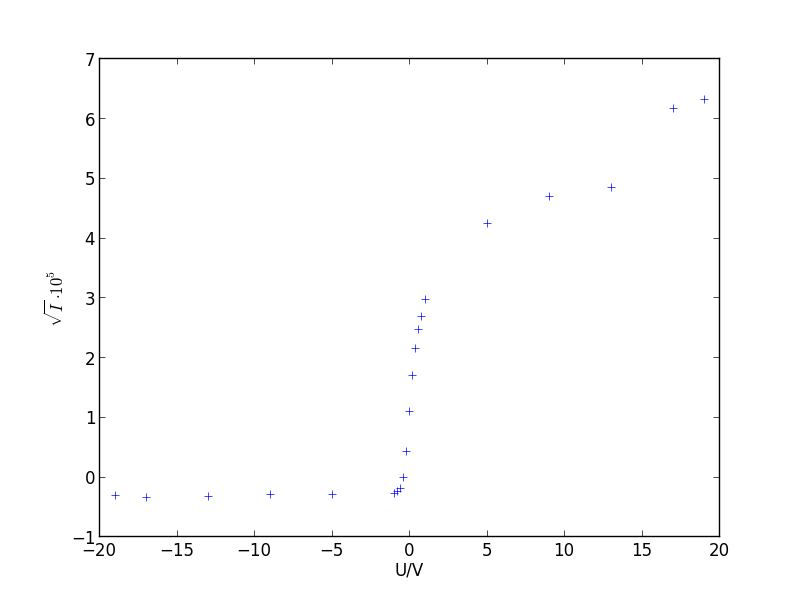
\includegraphics[scale=0.7]{picagelb.jpg}
		\caption{Photostrom in Abhängigkeit der angelegten Spannung ($\lambda=492$ nm)}
		\label{picagelb}
		\end{center}	
	\end{figure}
% In Abbildung \ref{picagelb} ist für $\lambda=578\text{ nm}$ der Photostrom abhängig der
% angelegten Spannung aufgetragen. Es ist bei hohen beschleunigenden Spannungen ein
% Sättigungsverhalten zu erkennen, dem zu Grunde liegt die Eigenschaft, dass die Anzahl der
% ausgelösten Elektronen von der Intesität des Lichtes abhängt. Das Ohmschen Gesetz lässt sich in diesem Fall 
% nicht anwenden, da die Elektronen zur Anode hin beschleunigt werden. Dieser Sättigungswert hängt neben
% der Intensität des Lichtes auch von der bestrahlten Fläche und den Materialeigenschaften ab. Dabei liegt 
% die Asymptotik an dem Unvermögen der Versuchsanordnung alle Elektronen zu registrieren, damit wirklich 
% alle Elektronen die Anode erreichen, müsste der Abstand zwischen Anode und Kathode gegen Null
% streben, was natürlich ein solches Experiment unmöglich machen würde.\\ 
% Der Photostrom nähert sich bereits bei $U>U_g$ an 0 V an, da die Elektronen nach der Fermi-Dirac 
% Statistik verteilt sind und es so auch Elektronen gibt, die bei $U>U_g$ gar nicht erst genug
% Energie besitzen die Anode zu erreichen. Der entgegengerichtete Photostrom von ungefähr -0,01 nA 
% kommt durch den an der Anode stattfindenden Photoeffekt zustande. Da die bestrahlte Oberfläche der 
% Anode wesentlich kleiner ist, wird schon bei relativ kleinen Spannungsbeträgen eine Sättigung erreicht.
% Die Austrittsarbeit der Anode ist gering, denn schon bei Einstrahlung energiearmen Lichtes 
% ($\lambda \approx 650$ nm)\cite{anleitung} tritt bereits ein negativer Photostrom auf.
	\FloatBarrier
\section{Diskussion}
	%
%

	\FloatBarrier
% ========================================
%	Literaturverzeichnis
% ========================================

\bibliographystyle{plainnat}			% Bibliographie-Style auswählen
\bibliography{lit}			% Literaturverzeichnis

% ========================================
%	Das Dokument endent
% ========================================
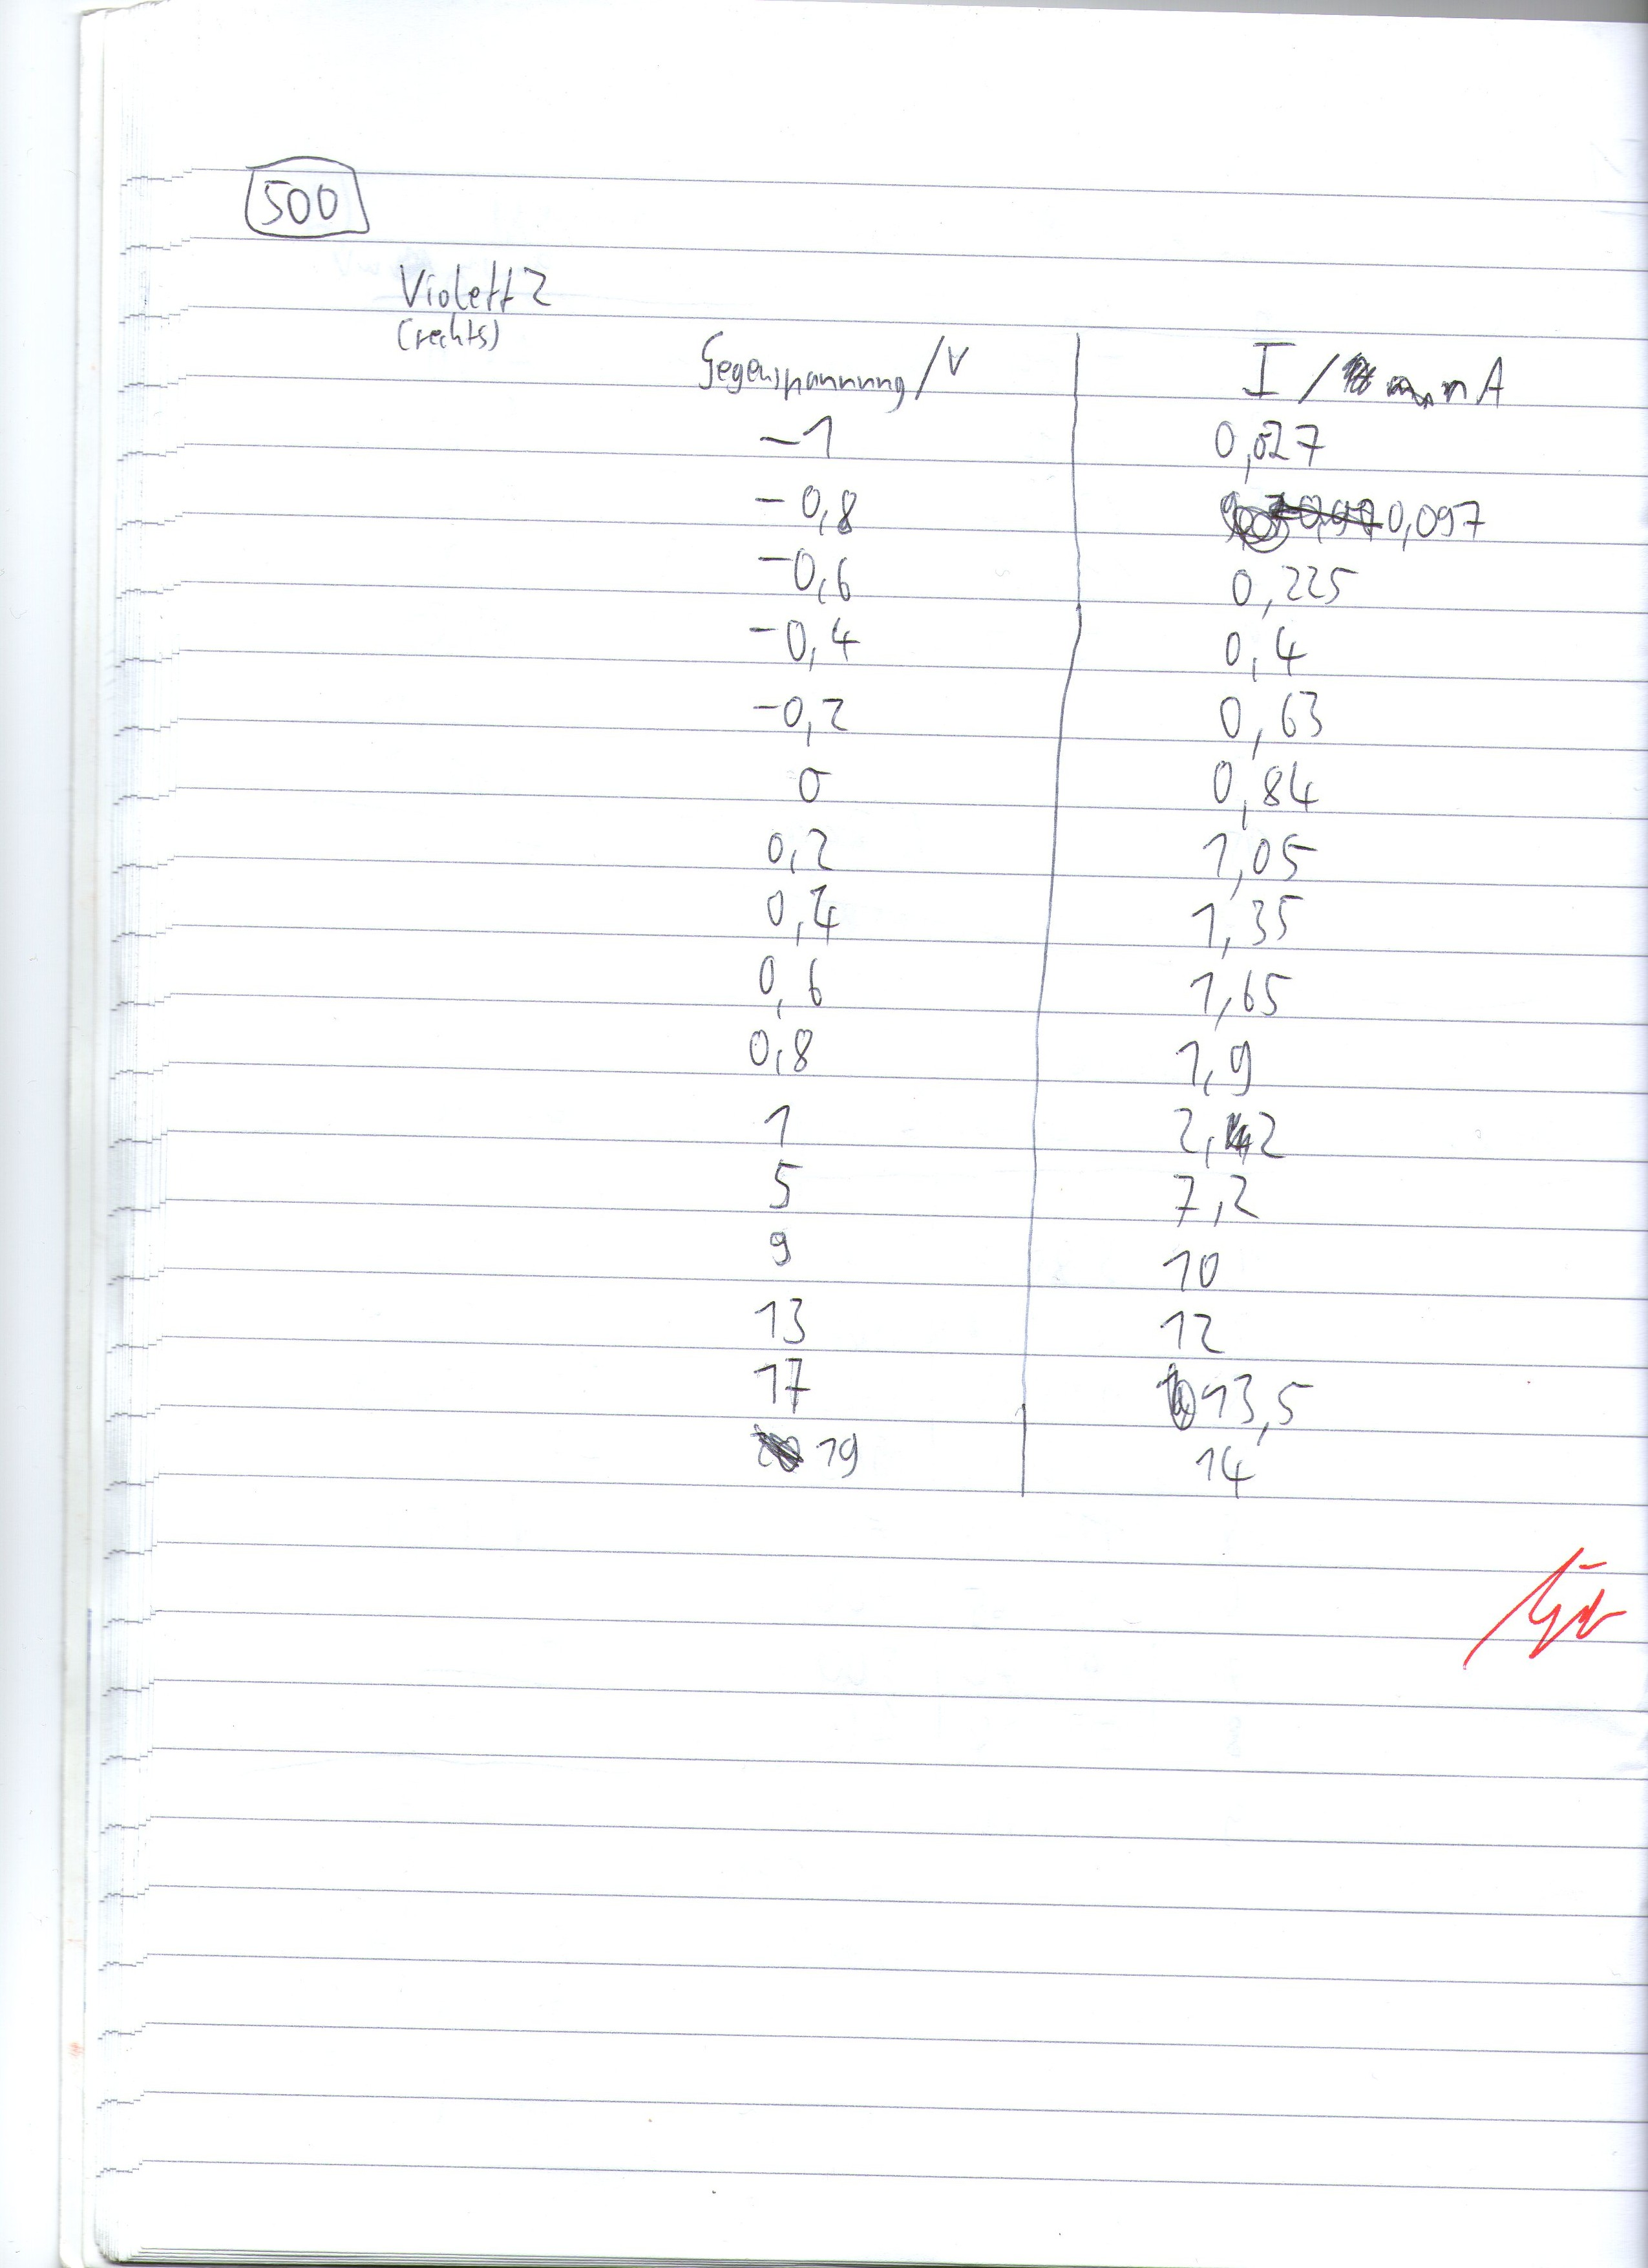
\includegraphics[scale=0.75]{img016.jpg}\\ \\
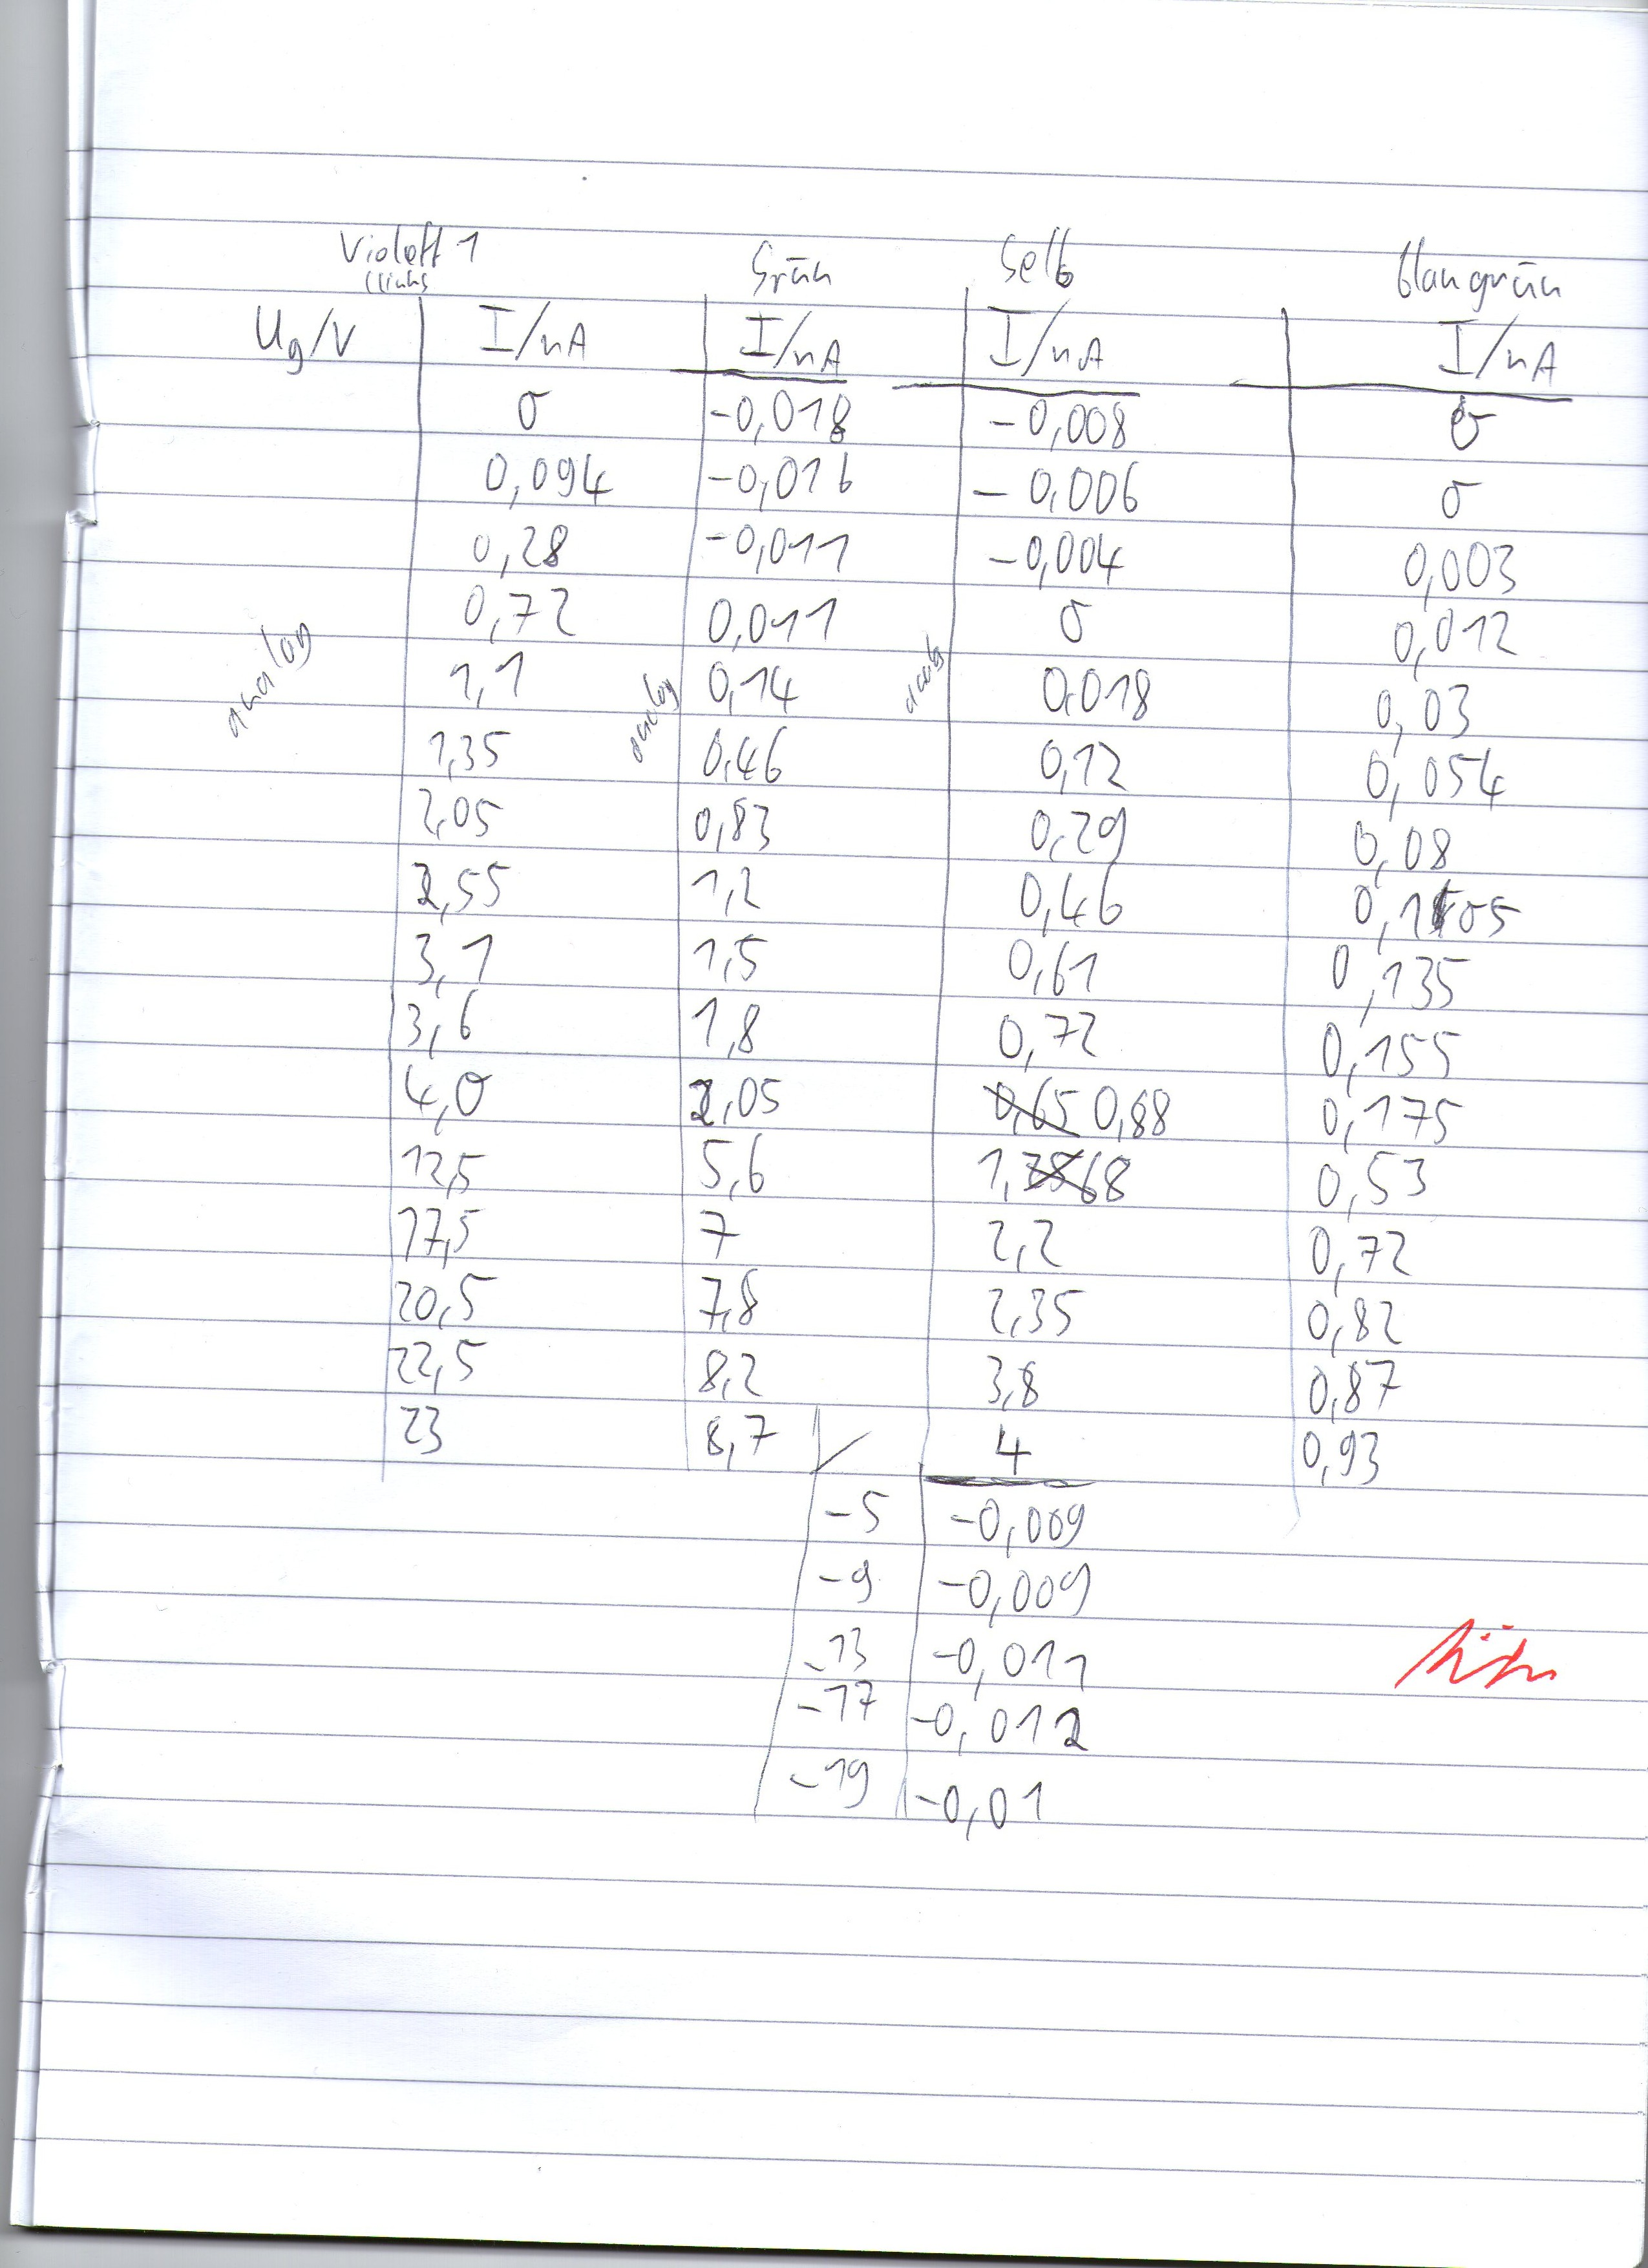
\includegraphics[scale=0.75]{img017.jpg}
\end{document}